\titledquestion{Huffman Coding}

After you compress a text file using Huffman Coding Algorithm, you accidentally spilled some ink on it and you found that one word becomes unrecognizable. Now, you need to recover that word given the following information:\\

\textbf{Huffman-Encoded sequence of that word: } \\
00001100111101\\
\textbf{Frequency table that stores the frequency of some characters: }\\
\begin{table}[!hbtp]
    \centering
    \begin{tabular}{|l|l|l|l|l|l|l|l|l|}
        \hline
        characters & b  & e & i & k & m & t & x \\ \hline
        frequency  & 12 & 9 & 6 & 7 & 2 & 1 & 5 \\ \hline
    \end{tabular}
\end{table}\\\\
\begin{parts}
    \part[4] Please construct the binary Huffman Coding Tree according to the given frequency table and draw the final tree below.\\
    Note: The initial priority queue is given as below. When popping nodes out of the priority queue, the nodes with the same frequency follows ``First In First Out".

    \begin{table}[!hbtp]
        \centering
        \begin{tabular}{|l|l|l|l|l|l|l|}
            \hline
            \begin{tabular}[c]{@{}l@{}}t\\ 1\end{tabular} & \begin{tabular}[c]{@{}l@{}}m\\ 2\end{tabular} & \begin{tabular}[c]{@{}l@{}}x\\ 5\end{tabular} & \begin{tabular}[c]{@{}l@{}}i\\ 6\end{tabular} & \begin{tabular}[c]{@{}l@{}}k\\ 7\end{tabular} & \begin{tabular}[c]{@{}l@{}}e\\ 9\end{tabular} & \begin{tabular}[c]{@{}l@{}}b\\ 12\end{tabular} \\ \hline
        \end{tabular}
    \end{table}

    \begin{solution}
        %\vspace{6.5cm}
        \begin{center}
            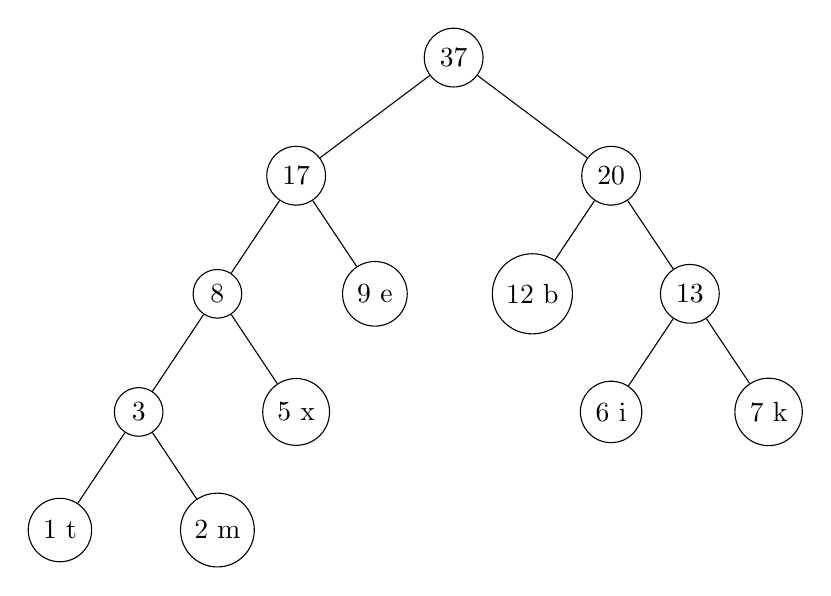
\begin{tikzpicture}[level distance=1.5cm,
                    level 1/.style={sibling distance=4cm},
                    level 2/.style={sibling distance=2cm},
                    every node/.style = {draw, circle}]
                \node {37}
                child { node {17}
                        child { node {8}
                                child { node {3}
                                        child { node {1 t} }
                                        child { node {2 m} }
                                    }
                                child { node {5 x} }
                            }
                        child { node {9 e} }
                    }
                child { node {20}
                        child { node {12 b}}
                        child { node {13}
                                child { node {6 i} }
                                child { node {7 k} }
                            }
                    };
            \end{tikzpicture}
        \end{center}
    \end{solution}

    \part[2] Now you can "decompress" the encoded sequence and recover the original word you lost. Please write the original word below.

    \begin{solution} \\
        %\vfill
        The word is tieke.
    \end{solution}

\end{parts}